% Generated from: Zhihu/专栏：概率与统计/渐近统计 (2) ：特征函数_金鱼马_2026-07-20.md
\section{特征函数的基本概念和性质}
\begin{definition}
  
对 $\mathbb R$ 上的随机变量 $X$ ，记其分布函数为 $F$ ，称复函数\[\phi_X(t)=\mathbb{E}\big[e^{itX}\big]=\int_{\mathbb R} e^{it x}\mathrm{d}F(x),\quad t\in\mathbb R\]
是 $X$ 的\textbf{\emph{特征函数}} (characteristic function)。
\end{definition}
\begin{remark}
  \begin{itemize}\tightlist
    \item 
由于 $\big|e^{it X}\big|\le 1$ ，因此\emph{特征函数一定存在}。
    \item 
    初学者必然会问：我们已经有矩母函数 (Moment Generating Function, MGF) $M_X(t) = \mathbb{E}[e^{tX}]$ 了，为什么还要引入带复数 $i$ 的特征函数？答案很简单，特征函数定义里的期望一定存在，但矩母函数不一定。例如对数正态分布就不存在矩母函数。

  \end{itemize}
\end{remark}

$\phi_X$ 的定义也可以称作是 $F$ 的 \textbf{\emph{Fourier-Stieltjes 变换}} 。如果 $X$ 存在密度函数 $F'=f$ 的话，那么 $\phi_X$ 本质上其上就是对密度函数 $f$ 的 Fourier 变换，因而提供了分布的频域视角。

部分常见分布的特征函数如下：\[\begin{array}{|c|c|} \hline \text{分布} & \text{特征函数}\\ \hline \text{退化分布 }\delta_a & e^{ita}\\ \hline \substack{\displaystyle\text{两点分布 }\\\text{(Bernoulli 分布)}}\mathrm{Ber}(p) & 1-p+pe^{it}\\ \hline \text{二项分布 }\mathrm{B}(n,p) & (1-p+pe^{it})^n\\ \hline \text{负二项分布 }\mathrm{NB}(r,p) & \left(\frac{p}{1+(1-p)e^{it}}\right)^r\\ \hline \text{Poisson 分布 }\mathrm{Pois}(\lambda) & e^{\lambda (e^{it}-1)}\\ \hline (a,b) \text{ 上的均匀分布 }\mathcal{U}(a,b) & \frac{e^{itb}-e^{ita}}{it(b-a)}\\ \hline \text{Laplace 分布 }\mathrm{Lap}(\mu,b) & \frac{e^{it\mu}}{1+b^2t^2}\\ \hline \text{Logistic 分布 }\mathrm{Logistic}(\mu,s) & e^{i\mu t}\frac{\pi st}{\sinh (\pi st)}\\ \hline \text{正态分布 }\mathcal{N}(\mu,\sigma^2) & e^{it\mu-\frac12\sigma^2t^2}\\ \hline k\text{ 个自由度的 }\chi^2\text{分布 } \chi_k^2& (1-it)^{-k/2}\\ \hline \text{Cauchy 分布 }\mathrm{Cauchy}(\mu,\theta) & e^{it\mu-\theta|t|}\\ \hline \text{指数分布 }\mathrm{Exp}(\lambda)& \left(1-\frac{it}\lambda\right)^{-1} \\ \hline \text{Gamma 分布 } \mathrm{Ga}(k,\lambda)& \left(1-\frac{it}\lambda\right)^{-k} \\ \hline \substack{ \displaystyle\text{几何分布 }\mathrm{Geom}(p) \\\text{(采用首次成功次数的定义)}}& \frac{p e^{it}}{1 - (1-p) e^{it}} \\ \hline \end{array}\]% 亦可见 \href{https://zhuanlan.zhihu.com/p/644138165}{常见分布的特征函数 - 知乎}。

可以表明，特征函数唯一确定分布：
\begin{theorem}[特征函数的唯一性]\label{thm:ch2:characteristic-uniqueness}

随机变量 $X,Y$ 同分布当且仅当 $\phi_X=\phi_Y$ 。
\end{theorem}

这个可以从 Fourier 变换的角度考虑：如果 $X$存在密度函数 $f$ ，并且 $\phi_X\in L^1(\mathbb R)$ （绝对可积），我们可以用 Fourier 反演从 $\phi_X$ 来唯一确定 $f$ ：

\begin{equation}
\label{eq:ch2:tag-1}
f(x)=\frac1{2\pi}\int_{\mathbb R}e^{-itx}\phi_X(t)\mathrm dt
\end{equation}

当然，更一般的情况下，``反演公式''的结论是这样的：对 $a<b$ 有

\begin{equation}
\label{eq:ch2:tag-2}
\lim_{T\to\infty}\frac1{2\pi}\int_{-T}^T\frac{e^{-ita}-e^{-itb}}{it}\phi_X(t)\mathrm{d}t=P(a<X<b)+\frac{P(X=a)+P(X=b)}2
\end{equation}

以及，

\begin{equation}
\label{eq:ch2:tag-3}
\lim_{T\to\infty}\frac1{2T}\int_{-T}^Te^{-ita}\phi_X(t)\mathrm{d}t=P(X=a)
\end{equation}

\begin{remark}

\begin{itemize}
\tightlist
\item
  这些公式的证明请参考 \cite{durrett2010} 的 Theorem 3.3.4 和 Theorem 3.3.5。
\item
  \eqref{eq:ch2:tag-2} 与 \eqref{eq:ch2:tag-3} 联合起来表明，若 $\phi_X=\phi_Y$ ，那么二者的分布在所有单点、以及开区间上都相同，自然是同一个分布。
\item
  在分布函数 $F$连续的情况下，式~\eqref{eq:ch2:tag-2} 右侧可以简化成 $F(b)-F(a)$ 。若其绝对连续，那么我们可以令 $a=x$ 、 $b=x+h$ 再让 $h\to 0$ ，两侧同时除以 $h$ ，就得到了式~\eqref{eq:ch2:tag-1}。
\end{itemize}
\end{remark}

鉴于分布和特征函数一一对应，很多时候与其直接研究分布 $F$ ，不如去研究 $\phi_X$ 来得容易一些。

特征函数的一些基本性质如下，都比较简单：

\begin{enumerate}
\def\labelenumi{\arabic{enumi}.}
\item
  $|\phi_X(t)| = |\mathbb{E}[e^{itX}]| \le \mathbb{E}[|e^{itX}|] = 1$；
\item
  $\overline{\phi_X(t)} = \phi_X(-t)$，即，特征函数是一个 Hermitian 函数。如果 $\phi_X$ 是一个实函数，那么 $X$ 的分布一定是对称的。
\item
  $\phi_{aX+b}(t)=e^{itb}\phi_X(at)$ 。
\item
  $\phi_X(t)$ 在 $\mathbb{R}$ 上一致连续；
\item
  $\overline{\phi_X}$、$|\phi_X|^2$ 和 $\operatorname{Re}(\phi_X)$ 分别是 $-X$、$X-Y$（其中 $X,Y$ 独立同分布于 $F$）以及对称化分布 $(F_X + F_{-X})/2$ 的特征函数。
\item
  若存在 $t_0 \neq 0$ 使得 $|\phi_X(t_0)| = 1$，则存在 $a \neq 0$ 和 $h=2\pi/|t_0|$ 使得 $P(X \in \{a + jh: j \in \mathbb{Z}\}) = 1$，即 $X$ 集中在格点上；
\item 
  $|\phi_X(t)|=1$ 对任意 $t$ 恒成立，当且仅当 $X$ 几乎必然是某个常数。
\item
  若 $F$ 绝对连续，则 $\lim_{|t|\to\infty} |\phi_X(t)| = 0$，这称作 \textbf{\emph{Riemann-Lebesgue 引理}}；
\item
  如果 $X,Y$ 独立，那么 $\phi_{X+Y}(t)=\phi_X(t)\phi_Y(t)$ ；
\end{enumerate}

\begin{remark}
  \begin{itemize}\tightlist
    \item 这里给出上述 (4.)(6.)(7.) 的证明。
    \begin{itemize}\tightlist
      \item[(4.)] 因为 
      \[      |\phi_X(t+h)-\phi_X(t)|=|\mathbb E[e^{i(t+h)X}-e^{itX}]|\le\mathbb E[|e^{i(t+h)X}-e^{itX}|]=\mathbb E[|e^{ihX}-1|]
      \]      用有界收敛定理交换极限和期望即证。
      \item[(6.)] 这是因为 $e^{it_0 X}$ 几乎必然是一个模 1 的复数，不妨记作 $e^{i\theta}$，于是 $t_0X-\theta\in 2\pi Z$ 几乎必然。
      \item[(7.)] 充分性显然，仅证明必要性。设 $|\phi_X(t)|=1$ 对任意 $t$ 恒成立，取 $X'$ 与 $X$ 同分布，则根据 (9.)， 
      \[      \mathbb E[e^{it (X'-X)}]=\phi_X(t)\phi_X(-t)=|\phi_X(t)|^2=1
      \]      即 $X'-X$ 的特征函数恒为 1，从而其几乎处处为 0；此时 $P(X'=X)=1$，对任意 Borel 集 $A$，
      \[      P(X\in A)=P(X\in A,X'\in A)=P(X\in A)^2\quad \implies \quad P(X\in A)=0\text{ 或 }1
      \]      即 $X$ 几乎必然是常数。
    \end{itemize}
    \item (9.) 是显然的：若 $X,Y$ 独立，则 $\mathbb E[e^{it(X+Y)}]=\mathbb E[e^{itX}]\mathbb E[e^{itY}]$。
    但要注意反过来是不成立的：$\phi_X(t)\phi_Y(t)=\phi_{X+Y}(t)$ 无法推出 $X,Y$ 独立。最简单的反例是取 $X$ 为标准 Cauchy 分布 $\mathrm{Cauchy}(0,1)$，$Y=X$。则
    \[
    \mathbb E[e^{it(X+Y)}]=\mathbb E[e^{2itX}]=e^{-|2t|},
    \]
    而
    \[
    \mathbb E[e^{itX}]\mathbb E[e^{itY}]
    =e^{-|t|}e^{-|t|}=e^{-|2t|}.
    \]
  \end{itemize}
\end{remark}
下面定义多维情形，

\begin{definition}  
如果 $X$ 是 $\mathbb R^k$ 上的随机向量，那么我们将特征函数定义为 $k$ 维复值函数，
\[
\phi_X(t)=\mathbb{E}[e^{it^\top X}]=\int_{\mathbb R^k}e^{it^\top x}\mathrm d x,\quad t\in\mathbb R^k.
\]
\end{definition}

% 前面一维情形的性质在高维的对应也均成立。

特别地， $k$ 维正态分布 $\mathcal{N}_k(\mu,\Sigma)$ 的特征函数是 $e^{it^\top\mu-\frac12t ^\top \Sigma t}$ 。

\section{Lévy 连续定理}

\textbf{\emph{Lévy 连续定理 }} 也是弱收敛的一个等价刻画，它表明：随机变量的弱收敛等价于其特征函数的逐点收敛。

\begin{theorem}[Lévy 连续定理]\label{thm:ch2:levy-continuity}

Lévy 连续定理：设 $X_n,X$ 是 $k$ 维随机向量，则 $X_n\overset{\rm d}\to X$ 当且仅当 $\phi_{X_n}(t)\to \phi_{X}(t)$ 对任意的 $t\in\mathbb R^k$ 成立。进一步，若 $\phi_{X_n}(t)$ 逐点收敛到某 $\phi$，且 $\phi$ 在 0 处连续，则 $\phi$ 也是某随机变量的特征函数。

\end{theorem}

\begin{proof}

由 $\phi_{X}$ 有界连续，若 $X_n\overset{\rm d}\to X$ ，则由 Portmanteau 定理的第 (2.) 条（见定理~\ref{thm:ch1:portmanteau}）， $\mathbb{E}[e^{it^\top X_n}]\to \mathbb{E}[e^{it^\top X}]$ 对任意的 $t$ 成立，这证明了必要性。

为了证明第二条叙述，考虑先证 $\{X_n\}$ 是胎紧的，再利用 Prohorov 定理（定理~\ref{thm:ch1:prohorov}）。

由于边际胎紧蕴含联合胎紧，只需证明每个分量是胎紧的，因此不失一般性设 $X_n$ 是一维随机变量。对任意 $x \in \mathbb{R}$ 和 $\delta > 0$，有如下不等式成立：\[\mathbb{I}(|\delta x| > 2) \le 2\left(1 - \frac{\sin \delta x}{\delta x}\right) = \frac{1}{\delta} \int_{-\delta}^{\delta} (1 - \cos t x) \mathrm dt\]图~\ref{fig:ch2:tail-bound} 直观展示了该不等式中两侧函数的关系。
\begin{figure}[htbp]
  \centering
  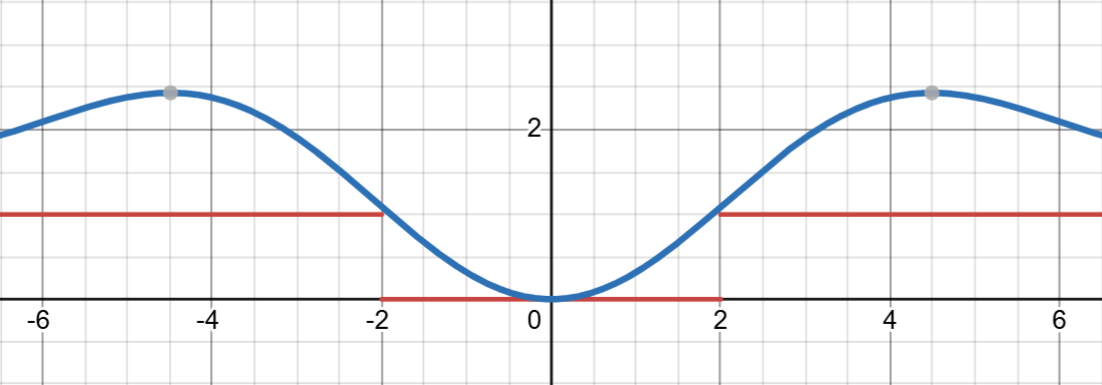
\includegraphics[width=0.82\textwidth]{figures/02-tail-bound-plot.png}
  \caption{$\mathbb I(|x|>2)$ 与 $2(1-\sin x/x)$ 的比较（Desmos 绘制）}
  \label{fig:ch2:tail-bound}
\end{figure}


这个不等式建立了``尾部概率''与``特征函数实部''之间的桥梁：将 $x$ 替换为随机变量 $X_n$，取期望并利用 Fubini 定理交换期望与积分得：\[P(|X_n| > 2/\delta) \le \frac{1}{\delta} \int_{-\delta}^{\delta} \mathbb{E}[1 - \cos(t X_n)] \mathrm{d}t = \frac{1}{\delta} \int_{-\delta}^{\delta} \operatorname{Re}\big(1 - \mathbb{E} [e^{i t X_n}]\big)  \mathrm{d}t\]
由假设，对每个 $t$，$\mathbb{E} [e^{i t X_n}] \to \phi(t)$，故上式中的被积函数逐点收敛到 $\operatorname{Re}(1 - \phi(t))$；利用控制收敛定理，当 $n \to \infty$ 时，\[\frac{1}{\delta} \int_{-\delta}^{\delta} \operatorname{Re}\big(1 -  \mathbb{E}[ e^{i t X_n}]\big)  \mathrm{d}t \to \frac{1}{\delta} \int_{-\delta}^{\delta} \operatorname{Re}(1 - \phi(t)) \mathrm{d}t\]
由于 $\phi$ 在零点连续，对任意 $\epsilon > 0$，存在 $\delta > 0$ 使得当 $|t| < \delta$ 时，$|1 - \phi(t)| < \epsilon$，从而 $\operatorname{Re}(1 - \phi(t)) \le |1 - \phi(t)| < \epsilon$。有\[\frac{1}{\delta} \int_{-\delta}^{\delta} \operatorname{Re}(1 - \phi(t))  \mathrm{d}t \le \frac{1}{\delta} \cdot 2\delta \epsilon = 2\epsilon\]
至此，我们表明了：对充分大的 $n$，\[P(|X_n| > 2/\delta) \le 2\epsilon\]
取 $M = 2/\delta$，则对任意 $\epsilon > 0$，存在 $M$ 和 $N$ 使得当 $n \ge N$ 时，$P(|X_n| > M) < 2\epsilon$ ，即得整个序列 $\{X_n\}$ 是胎紧的。

由 $\{X_n\}$ 胎紧，由 Prohorov 定理，取其任意子列，都可以在其中再抽出一个子列依分布收敛到某随机向量 $Y$。对该收敛子序列，其特征函数收敛到 $\phi$，故 $Y$ 的特征函数为 $\phi$ ，而特征函数唯一确定分布，因此所有可能的（弱收敛意义上的）极限点都有相同的分布，即整个序列 $\{X_n\}$ 只有唯一的极限点。这个推理足够表明 $X_n$ 本身依分布收敛到该极限------否则的话存在子列不收敛，矛盾！记该极限为 $X$，则 $X_n\overset{\rm d}\to X$ 且 $X$ 的特征函数为 $\phi$。

\end{proof}

值得一提的是，定理的必要性里，``逐点收敛''可以有加强的结论，

\begin{theorem*}

设 $X_n,X$ 是随机变量， $\phi_n,\phi$ 分别是其特征函数，若 $X_n\overset{\rm d}\to X$，那么 $\phi_n(t)\to \phi(t)$ 内闭一致收敛。

\end{theorem*}

\begin{proof}[证明概述]
Portmanteau 定理告诉我们 $\limsup\limits_{n\to \infty}P(|X_n|>M)\le P(|X|>M)$。因此，对任意 $t$ 和 $h$，
\[
\begin{aligned}
|\phi_n(t+h)-\phi_n(t)|
&\le\int_{\mathbb R}|e^{ihx}-1|\mathrm{d}F_n(x)\\
&\le \int_{|x|\le M}|hx|\mathrm{d}F_n(x)
 +2\int_{|x|>M}\mathrm{d}F_n(x)\\
&\le |h|M+2\int_{|x|>M}\mathrm{d}F(x)+\epsilon.
\end{aligned}
\]
上式对任意给定的 $\epsilon>0$、合适的 $M$ 以及足够大的 $n$ 成立。这证明了 $\{\phi_n\}$ 等度连续。剩下只需要在紧集上用经典的``$3\epsilon$''证明即可。
% ，例如，可参考文章 \url{https://zhuanlan.zhihu.com/p/347240346} 的定理 25。
\end{proof}

我们举两个简单的例子，以表 Lévy 连续定理是多么好用，

\begin{example}[Poisson 分布的中心极限定理]\label{ex:ch2:poisson-clt}
设随机变量 $X_1, \ldots, X_n$ 独立同分布于 $\operatorname{Poisson}(\lambda)$，其中 $\lambda > 0$ 固定，则它们的特征函数为 $\phi_X(t) = e^{\lambda(e^{it} - 1)}$ 。记样本均值 $\bar{X} = n^{-1}\sum_{i=1}^n X_i$，则标准化随机变量 $\frac{\bar{X} - \lambda}{\sqrt{\lambda/n}}$ 的特征函数为\[\begin{aligned} \phi_{\frac{\bar{X} - \lambda}{\sqrt{\lambda/n}}}(t) &= e^{-it\sqrt{n\lambda}} \phi_{\bar{X}}\!\left(\frac{t}{\sqrt{\lambda/n}}\right) = e^{-it\sqrt{n\lambda}} \left(\phi_X\!\left(\frac{t}{\sqrt{n\lambda}}\right)\right)^n \\ &= e^{-it\sqrt{n\lambda}} \exp\left\{n\lambda\left(e^{it/\sqrt{n\lambda}} - 1\right)\right\} \\ &= \exp\left\{-it\sqrt{n\lambda} + n\lambda\left(\frac{it}{\sqrt{n\lambda}} + \frac{(it)^2}{2n\lambda} + o\!\left(\frac{1}{n\lambda}\right)\right)\right\} \\ &= \exp\left\{-\frac{t^2}{2} + o(1)\right\} \\ &\to e^{-t^2/2},\quad \text{ 当 }n\to\infty \end{aligned}\]
这正是 $\mathcal{N}(0,1)$ 的特征函数！于是 Lévy 连续定理告诉我们\[\frac{\bar{X} - \lambda}{\sqrt{\lambda/n}} \overset{\rm d}\to \mathcal{N}(0,1)\]

\end{example}

\begin{example}[弱大数律]
设随机变量 $Y_1,Y_2,\dots,Y_n$ i.i.d.，其特征函数 $\phi_Y(t)$ 在 0 处可导，且 $\phi_Y'(0)=i\mu$ ，那么
\[
\bar Y=\frac1n\sum_{i=1}^nY_i\overset{p}\to \mu.
\]

我们知道，当极限是常数时，依分布收敛和依概率收敛是等价的（见定理~\ref{thm:ch1:convergence-relations} 的第 (3.) 条），只需证明 $\bar Y\overset{\rm d}\to \mu$ 。而由\[\phi_Y(t) = 1 + t\phi_Y'(0) + o(t), \quad t \to 0\]
有\[\phi_{\bar{Y}}(t) = \left(\phi_Y\!\left(\frac{t}{n}\right)\right)^n = \left(1 + \frac{t}{n}\phi'(0) + o\!\left(\frac{t}{n}\right)\right)^n = \left(1 + \frac{i t \mu}{n} + o\!\left(\frac{1}{n}\right)\right)^n \to e^{i t \mu}\]
依 Lévy 连续定理即得。


在下节中我们会表明，本例的 $\mu$ 正是总体均值。

\end{example}

\section{矩与特征函数}

\subsection{特征函数的展开}

这里请读者回忆 Fourier 变换的一个性质：时域函数的光滑程度直接决定了其频谱在高频区域的衰减速度，即，信号在时间上越平滑，其能量就越集中在低频部分，其高频成分消失得也越快。%可以参考 \href{https://www.zhihu.com/question/64361940}{关于Fourier transform的尾部decay rate的具体性质？}

对偶过来，时域的衰减速度也应该决定了频谱的光滑程度。有结论：若 $x^m f(x)\in L^1$ ，则 $f$ 的 Fourier 变换就是 $m$ 次可微的。

放在概率的语境下，$X$ 的分布对应``时域''，特征函数对应``频域''；应该说： $X$ 分布的尾部越薄， $\phi_X$ 就越光滑。根据 Markov 不等式， $P(|X|>x)\le \frac{\mathbb{E}[|X|^m]}{x^m},\,\forall x>0$ ， $\mathbb{E}[|X|^m]<\infty$ 对应于 $X$ 分布的尾部以至少 $x^{-m}$ 的速率衰减。我们可以用如下引理来描述，

\begin{lemma*}

设对于正整数 $m$ ，随机变量 $X$ 满足 $\mathbb{E}[|X|^m]<\infty$ ，那么其特征函数 $\phi_X$ 是 $m$ 次可导的，且其 $m$ 阶导数为
\[
\phi_X^{(m)}(t)=\mathbb{E}\big[(iX)^me^{itX}\big].
\]

特别地， $\phi_X^{(m)}(0)=\mathbb{E}\big[(iX)^m\big]$ 。

\end{lemma*}

\begin{proof}[证明简述]
利用 Lebesgue 控制收敛定理交换极限与积分，易得 $\phi'_X(t)=\mathbb{E}\big[(iX)e^{itX}\big]$，这个操作可以递推 $m$ 次。
\end{proof}

% \begin{remark}

% \begin{itemize}
% \tightlist
% \item
%   比较详细的证明可见 \href{https://www.zhihu.com/question/1987559971278304504/answer/1987590546710102543}{为什么随机变量的l阶矩存在就可以知道特征函数可求导？ - 知乎}；
% \item
%   这个结论同时告诉我们，对特征函数求 0 处 $m$ 阶导可以计算随机变量的 $m$ 阶矩。
% \end{itemize}
% \end{remark}
  这个结论同时告诉我们，对特征函数求 0 处 $m$ 阶导可以计算随机变量的 $m$ 阶矩。对 $\phi_X$ 在 0 处进行 Taylor 展开，可以得到如下定理：

\begin{theorem}[特征函数的 Taylor 展开]
\label{thm:ch2:characteristic-taylor}

设 $\mathbb{E}[|X|^m]<\infty$ ，则\[ \phi_X(t)=\sum_{j=0}^m\frac{(it)^j}{j!}\mathbb{E}[X^j]+o(|t|^m) \]

\end{theorem}

\begin{remark}

\begin{itemize}
\tightlist
\item
  由 Taylor 公式的 Lagrange 型余项，定理~\ref{thm:ch2:characteristic-taylor} 也可以写成：
  \[  \phi_X(t)=\sum_{j=0}^{m-1}\frac{(it)^j}{j!}\mathbb{E}[X^j]+\frac{\lambda |t|^m}{m!}\mathbb{E}[|X|^m],
  \]  其中复数 $|\lambda|\le 1$ 。
\item
  定理~\ref{thm:ch2:characteristic-taylor} 的余项可以由如下不等式控制：
  \[  \left|e^{ix}-\sum_{m=0}^n\frac{(ix)^m}{m!}\right|\leq\min\left(\frac{|x|^{n+1}}{(n+1)!},\frac{2|x|^n}{n!}\right).
  \]  见 \cite{durrett2010}, Lemma 3.3.7。因此
  \[  \left| \phi_X(t) - \sum_{j=0}^m \frac{(it)^j}{j!}\mathbb{E}[X^j] \right| \leq \mathbb{E}\left[ \left| e^{itX} - \sum_{j=0}^m \frac{(itX)^j}{j!} \right| \right] \leq \mathbb{E}\left[ \min\left\{ \frac{|tX|^{m+1}}{(m+1)!}, \frac{2|tX|^m}{m!} \right\} \right].
  \]\end{itemize}
\end{remark}

\subsection{中心极限定理}

仿照例~\ref{ex:ch2:poisson-clt}，我们可以证明一般的中心极限定理：

\begin{example}[中心极限定理]\label{ex:ch2:clt}
设 $X_1, \ldots, X_n$ 是 $\mathbb R$ 上 i.i.d. 的随机变量，有均值 $\mathbb{E}[X_1]=\mu$ 和方差 $\mathbb{E}[(X_1-\mu)^2]=\sigma^2$，其中 $-\infty<\mu<\infty$、$0<\sigma^2<\infty$，则\[\frac{\bar{X} - \mu}{\sqrt{\sigma^2/n}} \xrightarrow{\rm d} \mathcal{N}(0,1)\]
\begin{proof}

将 $X_1,X_2,\dots$ 中心化后的特征函数记为 $\phi_{X-\mu}$，则当 $n\to\infty$，\[\phi_{ \frac{\bar{X} - \mu}{\sqrt{\sigma^2/n}} }(t) = \left(\phi_{X-\mu}\!\left(\frac{t}{\sigma\sqrt{n}}\right)\right)^n = \left(1 - \frac{1}{2}\left(\frac{t}{\sigma\sqrt{n}}\right)^2 \sigma^2 + o\!\left(\frac{t^2}{\sigma^2 n}\right)\right)^n \to e^{-t^2/2}.\]依 Lévy 连续定理即得。

\end{proof}

例~\ref{ex:ch2:clt} 的这个结论也可以写作 $\frac{1}{\sqrt n}\sum_{j=1}^n(X_i-\mu)\overset{\rm d}\to \mathcal{N}(0,\sigma^2)$ 。

\end{example}

\begin{theorem}[Cramér--Wold 定理]\label{thm:ch2:cramer-wold}

设 $\{X_n\}_{n=1}^\infty$ 是一列 $\mathbb R^k$ 上的随机向量，那么\[X_n\overset{\rm d}\to X\ \iff \ c^\top X_n\overset{\rm d}\to c^\top X,\enspace \forall c\in\mathbb R^k\]
即，高维随机向量的依分布收敛等价于其任意方向上的``投影''或者说``边际 (marginal)''的依分布收敛。

\end{theorem}

\begin{proof}

`` $\Longrightarrow$ ''根据连续映射定理是显然的，只需证明`` $\Longleftarrow$ ''。设 $X_n=(X_{n1},\dots,X_{nk})^\top$ 、 $X=(X_1,\dots,X_k)^\top$ ，二者的特征函数分别为 $\phi_n$ 和 $\phi$ 。对于任意的 $c=(c_1,\dots,c_k)^\top\in\mathbb R^k$ ，由假设，\[c_1X_{n1}+\cdots+c_kX_{nk}\overset{\rm d}\to c_1X_1+\cdots +c_kX_k,\quad \text{当 }n\to\infty\]
根据 Lévy 连续定理，上式等价于特征函数的逐点收敛：\[\mathbb{E}\left[e^{it(c_1X_{n1}+\cdots+c_kX_{nk})}\right]\to \mathbb{E}\left[e^{it(c_1X_{1}+\cdots+c_kX_{k})}\right]\]
亦即，
\[
\phi_n(tc_1,tc_2,\dots,tc_n)\to \phi(tc_1,tc_2,\dots,tc_n).
\]

对任意 $t\in\mathbb R$ 成立，取 $t=1$ 即可看出 $\phi_n(c)\to \phi(c),\,\forall c\in\mathbb R^k$ ，从而 $X_n\overset{\rm d}\to X$ 。

\end{proof}

\begin{remark}

\begin{itemize}
\tightlist
\item
  给该定理一个引用出处：\cite{serfling1980} 的 p.18。
\item
  特别地，要证明 $X_n$ 依分布收敛于正态分布，只需要证明对任意的 $t$ 有$t^\top X_n$ 依分布收敛于正态分布；这是因为 $X$ 是多维正态分布当且仅当其每个边际 $t^\top X$ 都是一维正态分布 (e.g., 见 \cite{vershynin2018} 的 Exercise 3.3.4)
\end{itemize}
\end{remark}

\begin{example}[高维中心极限定理]
设 $Y_1,Y_2,\dots,Y_n$ 是 $\mathbb R^k$ 上的 i.i.d. 随机向量，有均值向量 $\mathbb{E}[Y_1]=\mu$ 和协方差矩阵 $\mathbb{E}[(Y_1-\mu)(Y_1-\mu)^\top]=\Sigma$，则 $\frac1{\sqrt n}\sum_{j=1}^n(Y_j-\mu)=\sqrt n(\bar Y-\mu)\overset{\rm d}\to \mathcal{N}(0,\Sigma)$。

\begin{proof}
用 Cramér--Wold 定理化为一维情形。注意到 $t^\top Y_1-t^\top \mu$、$t^\top Y_2-t^\top \mu$、\ldots{} 是 i.i.d. 的、均值为 0、方差为 $t^\top\Sigma t$ 的随机变量，用例~\ref{ex:ch2:clt} 结论，$t^\top\left(\frac1{\sqrt n}\sum_{j=1}^n(Y_j-\mu)\right)=\frac1{\sqrt n}\sum_{j=1}^n(t^\top Y_j-t^\top \mu)\overset{\rm d}\to \mathcal{N}(0,t^\top\Sigma t)$。
\end{proof}

\end{example}

\subsection{矩问题}

一个自然的问题是：既然特征函数完全决定了分布的矩，那么，仅通过分布的矩能否反过来确定分布？

答案是否定的，我们这里仅简略介绍一下。它被称作``\textbf{\emph{矩问题}} (moment problem)''。一个反例 (来自 \cite{heyde1963}) 是对数正态分布，其密度为 $f_0(x)=(2\pi)^{-1/2}x^{-1}e^{-(\log x)^2/2}$ ，以及一个``扰动分布''，其密度为 $f_a(x)=f(x)(1+a\sin(2\pi\log x))$ ，二者拥有相同的各阶原点矩。

记 $\alpha_m:=\mathbb{E}[X^m]$ 为原点矩，若如下的``\textbf{\emph{Carleman 条件}}''成立：\[ \sum_{m=1}^\infty \alpha_{2m}^{-\frac1{2m}}=\infty \]则 $\{\alpha_m\}$ 唯一确定 $X$ 的分布。

直觉上可以理解为，如果分布尾部较厚， $\alpha_{2m}$ 就会增长得很快，那么 $\alpha_{2m}^{-\frac1{2m}}$ 下降得也很快，其求和就会更可能收敛，分布的``唯一性''越弱，导致不同的分布可以拥有完全相同的一组矩；反过来，如果分布尾部较薄， $\alpha_{2m}$ 的增长、以及 $\alpha_{2m}^{-\frac1{2m}}$ 的下降也都会放慢，求和才更偏向于发散，分布的``唯一性''就越强。

Carleman 条件的证明依赖于 Denjoy--Carleman 关于实值函数拟解析性（quasi-analyticity）的定理，不再赘述。
% ，可参考这篇文章的定理11：
% \href{https://zhuanlan.zhihu.com/p/1986628306896962819}{谈概率分布的收敛}
关于矩问题，亦可参阅 \cite{durrett2010} 的 §3.3.6，或者更深入讨论的文献 \cite{schmudgen2017}。

\section{Edgeworth 展开}

中心极限定理告诉我们 $\sqrt{n}(\bar X-\mu)/\sigma$ 依分布收敛于标准正态分布，但这个收敛有多快？对于给定的 $n$ ，近似的误差有多大？以及能否通过修正项提高精度？Edgeworth 展开正是这样一种工具：它将标准化和的分布渐近展开为 $\Phi(x)$ 加上若干修正项，这些修正项由 $X$ 的高阶矩（偏度、峰度等）决定。

对随机变量 $X$ ，我们记其 $m$ 阶原点矩为 $\alpha_m=\mathbb{E}[X^m]$ （特别地， $\alpha_1=\mu$ ），其 $m$ 阶中心矩为 $\mu_m:=\mathbb{E}[(X-\mu)^m]$ （特别地， $\mu_1=0$ 、 $\mu_2=\sigma^2$ ）。$\Phi,\varphi$ 分别是标准正态分布 $\mathcal N(0,1)$ 的分布函数和密度函数。

若对 $m=1,2,\dots$ ， $\mathbb R$ 上随机变量 $X$ 满足 $\mathbb{E}[|X|^m]<\infty$ ，那么根据定理~\ref{thm:ch2:characteristic-taylor}，
\[
\phi_{X-\mu}(t) = 1 + \frac{1}{2}(it)^2\mu_2 +\frac{1}{6}(it)^3 \mu_3 +\cdots + \frac{1}{m!} (it)^m\mu_m + o(|t|^m).
\]

于是，若 $X_1,\dots,X_n$ i.i.d.与 $X$ 同分布，则\[\phi_{\frac{\bar{X}-\mu}{\sqrt{\sigma^2/n}}}(t) = \left(\phi_{X-\mu}\!\left(\frac{t}{\sigma\sqrt{n}}\right)\right)^n = \left(1 - \frac{t^2}{2n} - \frac{i t^3}{6 n^{3/2}} \frac{\mu_3}{\sigma^3} + \frac{t^4}{24 n^2} \frac{\mu_4}{\sigma^4} + \cdots\right)^n.\]
看起来要展开这个式子似乎有些麻烦？

我们想到：可以用对数来将幂化作求和形式。这是一个非常简单直接的技巧：如果 $X$ 和 $Y$ 是独立的随机变量，它们的特征函数相乘 $\phi_{X+Y}(t) = \phi_X(t)\phi_Y(t)$；一旦取了对数，乘法就变成了加法：$\log \phi_{X+Y}(t) = \log \phi_X(t) + \log \phi_Y(t)$。

定义如下概念：对随机变量 $X$ ，称 $\log \phi_X(t)=\log\mathbb{E}[e^{itX}]$ 为其\textbf{\emph{累积生成函数}} (cumulant generating function, CGF)，其 Taylor 展开 \[ \log \phi_X(t)=\sum_{j=1}^\infty \kappa_j\frac{(it)^j}{j!} \]中的各次数 $\kappa_1,\kappa_2,\dots$ 则称作\textbf{\emph{累积量}} (cumulant)。累积量和矩非常类似，也能够提供和矩一样的信息，不难算出：

\begin{itemize}
\tightlist
\item
  $\kappa_1=\frac{{\rm d}\log \phi_X}{\mathrm{d}t}(0)=\frac{\phi'_X(0)}{\phi_X(0)}=\mathbb{E}[X]=\alpha_1$ ;
\item
  $\kappa_2=\frac{{\rm d}^2\log \phi_X}{\mathrm{d}t^2}(0)=\frac{\phi''_X(0)\phi(0)-(\phi'(0))^2}{(\phi_X(0))^2}=\mathbb{E}[X^2]-(\mathbb{E}[X])^2=\alpha_2-\alpha_1^2=\mu_2$ ;
\item
  $\kappa_3=\frac{{\rm d}^3\log\phi_X}{\mathrm{d}t^3}=\alpha_3-3\alpha_2\alpha_1+2\alpha_1^3=\mu_3$ ;
\item
  $\kappa_4=\frac{{\rm d}^4\log \phi_X}{\mathrm{d}t^4}(0)=\alpha_4-4\alpha_3\alpha_1-3\alpha_2^2+12\alpha_2\alpha_1^2-6\alpha_1^4=\mu_4-3\mu_2^2$ ;
\item
  \ldots{}
\end{itemize}

按此继续，例如 $\kappa_{10}$ 可以写成多达 41 项相加。

对于归一化的随机变量 $Y=\frac{X-\mu}{\sigma}$ ，它的前四个累积量是 $\kappa_1=0$ 、 $\kappa_2=1$ 、 $\kappa_3=\frac{\mathbb{E}[(X-\mu)^3]}{\sigma^3}$ 称作 $X$ 的\textbf{\emph{偏度}} (Skewness)、 $\kappa_4=\frac{\mathbb{E}[(X-\mu)^4]}{\sigma^4}-3$ 称作 $X$ 的\textbf{\emph{峰度}} (Kurtosis)。于是\[ \phi_Y(t) = \exp \left\{ \sum_{j = 1}^\infty \frac{(it)^j}{j!} \kappa_j \right\} = \exp \left\{ -\frac{t^2}{2} + \sum_{j = 3}^\infty \frac{(it)^j}{j!} \kappa_j \right\} \]从而，若 $X_1,\dots,X_n$ i.i.d.与 $X$ 同分布，记 $S_n:=\frac{\bar{X}-\mu}{\sqrt{\sigma^2/n}}$ ，则有\[\begin{aligned} \phi_{S_n}(t) &= \left(\phi_Y\left(\frac{t}{\sqrt{n}}\right)\right)^n \\ &= \exp\left\{ -\frac{t^2}{2} + \sum_{j = 3}^\infty \kappa_j \frac{(it)^j}{j!} n^{-\frac{j-2}{2}} \right\} \\ &=e^{-\frac{t^2}{2}}\left(1+\sum_{m=1}^\infty\frac1{m!}\left(\sum_{j=3}^\infty\kappa_j \frac{(it)^j}{j!} n^{-\frac{j-2}{2}} \right)^m\right)\\ &= e^{-\frac{t^2}{2}} \left( 1 + \sum_{j = 1}^\infty n^{-\frac{j}{2}} r_j(it)\right) \end{aligned}\]
其中 $r_j$ 是次数为 $3j$ 的实系数多项式，依赖于 $\kappa_3,\dots,\kappa_{j+2}$ 但不依赖于 $n$ ；如

\begin{itemize}
\tightlist
\item
  $r_1(u)=\frac16\kappa_3u^3$ ;
\item
  $r_2(u)=\frac1{24}\kappa_4 u^4+\frac1{72}\kappa_3^2u^6$ ;
\item
  \ldots{}
\end{itemize}

至此，我们得到了这样的结论

\begin{equation}
\label{eq:ch2:tag-4}
\phi_{S_n}(t)=e^{-\frac{t^2}2}\left(1+n^{-1/2}r_1(it)+n^{-1}r_2(it)+\cdots++n^{-j/2}r_j(it)+\cdots\right)
\end{equation}

上面的第一项正是标准正态分布的特征函数！对比 \[ \phi_{S_n}(t) = \int_{-\infty}^\infty e^{itx}\,\mathrm dP(S_n \leq x), \quad e^{-t^2/2} = \int_{-\infty}^\infty e^{itx}\,\mathrm d\Phi(x) \]则 式~\eqref{eq:ch2:tag-4}向我们传达了一个信息：

\begin{equation}
\label{eq:ch2:tag-5}
P(S_n\le x)=\Phi(x)+n^{-1/2}R_1(x)+n^{-1}R_2(x)+\cdots+n^{-j/2 }R_j(x)+\cdots
\end{equation}

其中 $R_j(x)$ 是一个 Fourier-Stieltjes 变换是 $e^{-\frac{t^2}2}r_j(it)$ 的函数，亦即，\[\int_{\mathbb R}e^{itx}\mathrm{d}R_j(x)=e^{-\frac{t^2}2}r_j(it)\]
下一步，我们的目标就变成了确定 $R_j$ 。由分部积分，\[\begin{aligned}  e^{-t^2/2} &= \int_{-\infty}^\infty  e^{itx}\,\mathrm d\Phi(x)\\ & =(-it)^{-1}\int_{-\infty}^{\infty}e^{itx}\mathrm d\Phi'(x) \\   & =(-it)^{-2}\int_{-\infty}^{\infty}e^{itx}\mathrm d\Phi''(x) \\   \vdots\\   & =-(-it)^{-j}\int_{-\infty}^{\infty}e^{itx}\mathrm d\Phi^{(j)}(x) \end{aligned}\]
可以看出
\[
\int_{-\infty}^\infty e^{itx}\mathrm{d}((-D)^j\Phi(x))
=(it)^je^{-t^2/2},
\]
其中 $D=\frac{\mathrm d}{\mathrm dx}$ 是微分算子。我们把多项式 $r_j$ 作用在 $-D$ 上，得到 $r_j(-D)$ （这本身仍然是一个微分算子），于是上式表明\[\int_{-\infty}^\infty e^{itx}\mathrm{d}(r_j(-D)\Phi(x))=r_j(it)e^{-\frac{t^2}2}\]
我们想找的 $R_j$ 就此现身！由式~\eqref{eq:ch2:tag-5} 立即推出 $R_j(x)=r_j\left(-D\right)\Phi(x)$

此外，Hermite 多项式定义为
\[
\mathrm{He}_n(x):=(-1)^ne^{x^2/2}\frac{\mathrm{d}^n}{\mathrm{d}x^n}e^{-x^2/2}.
\]
这是一个 $n$ 次的实系数首一多项式：

\begin{itemize}
\tightlist
\item
  $\mathrm{He}_0(x)=1$ ;
\item
  $\mathrm{He}_1(x)=x$ ;
\item
  $\mathrm{He}_2(x)=x^2-1$ ;
\item
  $\mathrm{He}_3(x)=x^3-3x$ ;
\item
  $\mathrm{He}_4(x)=x^4-6x^2+3$ ;
\item
  $\mathrm{He}_5(x)=x^5-10x^3+15x$ ;
\item
  \ldots{}
\end{itemize}

并且满足 $(-D)^j\varphi(x)=\mathrm{He}_{j}(x)\varphi(x)$；那么当 $j\ge 1$ 时，
\[
(-D)^j\Phi(x)=-\mathrm{He}_{j-1}(x)\varphi(x).
\]
据此可以具体算出 $R_j(x)$，

\begin{itemize}
\tightlist
\item
  $R_1(x)=r_1(-D)\Phi(x)=\frac16\kappa_3(-D)^3\Phi(x)=-\frac16\kappa_3(x^2-1)\varphi(x)$ ;
\item
  \[
  \begin{aligned}
  R_2(x)&=r_2(-D)\Phi(x)\\
  &=\left(\frac1{24}\kappa_4 (-D)^4\Phi(x)+\frac1{72}\kappa_3^2(-D)^6\Phi(x)\right)\\
  &=-\left(\frac1{24}\kappa_4(x^3-3x)+\frac1{72}\kappa_3^2(x^5-10x^3+15x)\right)\varphi(x).
  \end{aligned}
  \]
\item
  \ldots{}
\end{itemize}

一般地，可以写作 $R_j(x)=p_j(x)\varphi(x)$ ，其中 $p_j$ 是一个 $3j-1$ 次多项式。 式~\eqref{eq:ch2:tag-5}便可写作\[P(S_n\le x)=\Phi(x)+n^{-1/2}p_1(x)\varphi(x)+n^{-1}p_2(x)\varphi(x)+\cdots+n^{-j/2 }p_j(x)\varphi(x)+\cdots\]
这就是 \textbf{\emph{Edgeworth 展开 }} (Edgeworth expansion)。

Edgeworth 展开往往只有\emph{渐近展开}的意义，即其描述的是 $n\to\infty$ 时的行为。使用 Edgeworth 展开时，最常用到的一个条件称作 \textbf{\emph{Cramér 条件 }}：如果 $X$ 满足 $\mathbb{E}[|X|^{j+2}]<\infty$ 且 $\limsup\limits_{|t|\to\infty}|\phi_X(t)|<1$ ，则可以将 Edgeworth 展开写到第 $j+1$ 项：\[P(S_n\le x)=\Phi(x)+n^{-1/2}p_1(x)\varphi(x)+n^{-1}p_2(x)\varphi(x)+\cdots+n^{-j/2 }p_j(x)\varphi(x)+o(n^{-j/2}),\quad \text{ 当 }n\to\infty\]
它的重要意义在于\emph{提供了中心极限定理的修正 }，并且，如果能够获得总体分布的三阶或更高阶矩的信息，则可以获得更高阶的修正项，因此，它常常用于提高统计量的收敛速度或提升统计推断的准确性。例如，Bootstrap 的正确性和 Edgeworth 展开有很大的关系，经典著作 \cite{hall1992} 就详细介绍了此事。

\begin{example}[指数分布的 Edgeworth 展开]
这个例子来自于 \href{https://gregorkb.github.io/nonparm/edgeworthplay.html}{Karl Gregory}。设 $X_1,\dots,X_n$ i.i.d. 服从指数分布 $\mathrm{Exp}(\lambda)$ ，那么，总体均值为 $\mathbb{E}[X_1]=1/\lambda$ 、方差 $\mathrm{Var}[X_1]=1/\lambda^2$ ，峰度和偏度分别是 $\kappa_3=2$ 和 $\kappa_4=6$。记
\[
S_n:=\sqrt n\frac{\bar{X}-1/\lambda}{1/\lambda},
\]
则它的分布为 $\mathrm{Ga}(n,n^{1/2})-\sqrt n$。考虑用 Edgeworth 展开近似这个分布：

\begin{itemize}
\tightlist
\item
  0 阶： $\Phi(x)$ ；
\item
  1 阶： $\widetilde{F}_{S_n}^{(1)}(x) =\Phi(x) - \frac{1}{3\sqrt{n}} (x^2 - 1) \varphi(x)$ ；
\item
  2 阶： $\widetilde{F}_{S_n}^{(2)}(x) = \widetilde{F}_{S_n}^{(1)}(x) - \frac{1}{n}\left(\frac{1}{4}(x^3 - 3x) + \frac{1}{18} (x^5 - 10x^3 + 15x) \right) \varphi(x)$ 。
\end{itemize}

取 $n=6$ 时的结果如图~\ref{fig:ch2:edgeworth-exponential} 所示：

\begin{figure}[htbp]
  \centering
  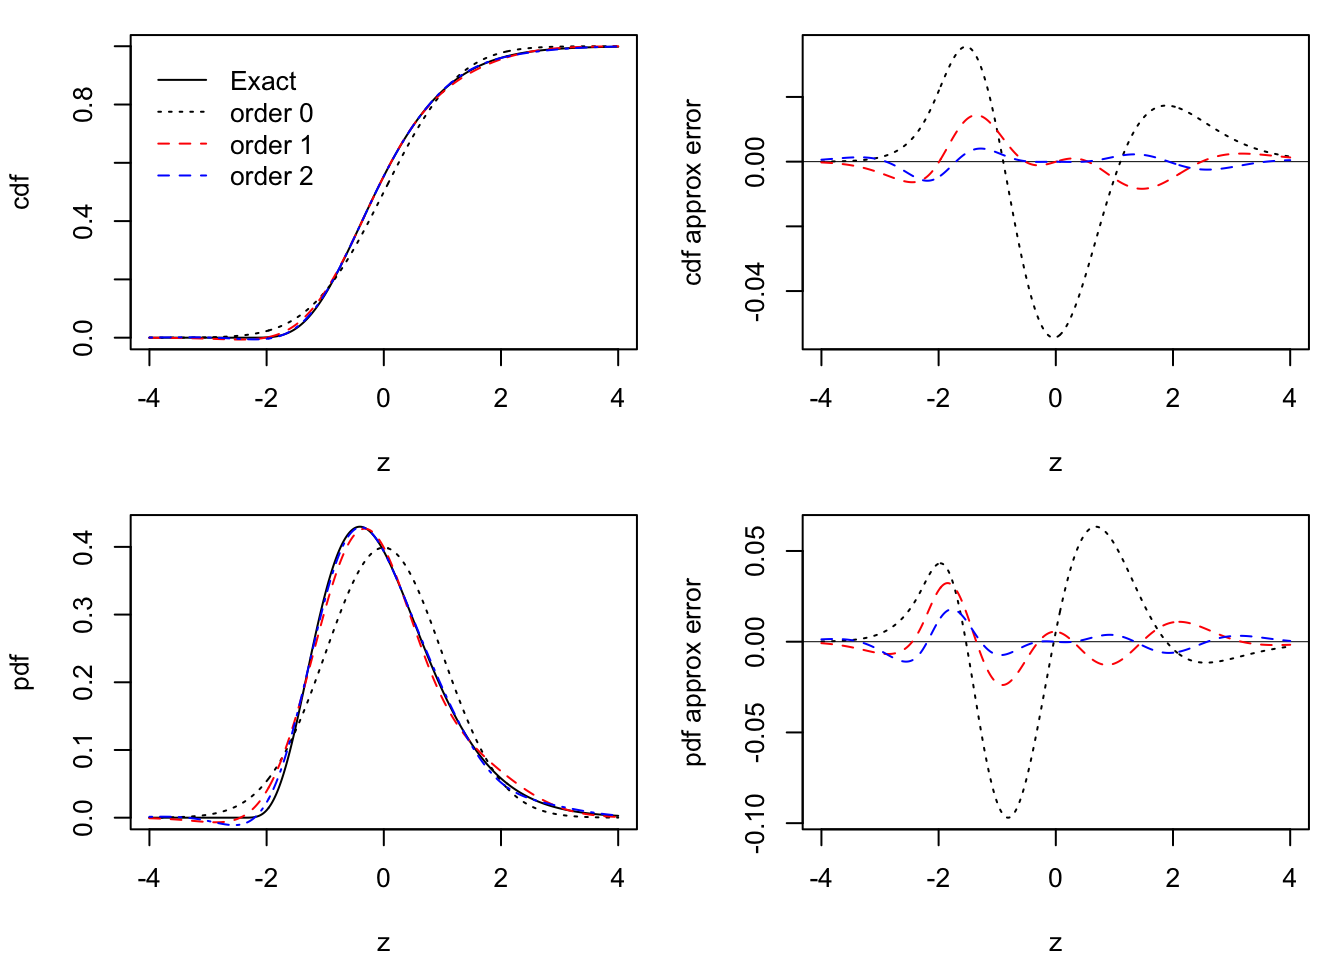
\includegraphics[width=0.88\textwidth]{figures/02-edgeworth-expansion.png}
  \caption{$n=6$ 时指数分布标准化样本均值的 Edgeworth 近似；图片来自 \url{https://gregorkb.github.io/nonparm/edgeworthplay.html}}
  \label{fig:ch2:edgeworth-exponential}
\end{figure}

\end{example}


% Karl Gregory 的博客内容清晰生动、深入浅出，可以去看一看： \url{https://gregorkb.github.io/nonparm/edgeworth.html}、\url{https://gregorkb.github.io/nonparm/edgeworthplay.html}、\url{https://gregorkb.github.io/nonparm/edgeworthmulti.html}、\url{https://gregorkb.github.io/nonparm/edgeworthboot.html}。

Edgeworth 展开解决的是正向问题：``已知分位点 $x$，求更精确的概率分布 $P(S_n \le x)$''。而在实际中，也会遇到需要反向操作的情况：``已知概率 $\alpha$，求更精确的分位数 $x_\alpha$''；这种情况下，将 Edgeworth 展开``反转''，可以得到著名的 \textbf{\emph{Cornish-Fisher 展开}} ，我们会在~\ref{sub:ch11b:cornish-fisher} 中详细说明。

还有要指出的是，读者可能了解``描述中心极限定理的收敛''的另一个结论：\textbf{\emph{Berry-Essen 界}} ， $|F_{S_n}(x)-\Phi(x)|\le \frac{C\mathbb{E}[|X_1-\mu|^3]}{\sigma^3\sqrt n},\quad \forall x\in\mathbb R,\forall n$Berry-Essen 界的优点在于它是一个一致的误差界，但它无法提供中心极限定理的修正信息，是做不到纠偏的。 Edgeworth 展开可以明确将误差分解为 $n^{-1/2}, n^{-1}, \dots$ 项，从而构造出更精确的逼近。

最后，高维情形下 Edgeworth 展开的核心逻辑是不变的，但实际写起来非常非常的繁琐：这需要将累积量 $\kappa_j$ 推广到 $\phi_X(t)$ 在 0 处的多元 Taylor 级数的系数，还要定义高维的 Hermite 多项式。当维数增大时，展开式中的项数会爆炸式增长。由于复杂性，其在实际数据分析中的直接应用不如一维广泛，我们这里不再细述。
